\subsection{Hardware/Software mapping}
\paragraph{Systems}\mbox{}\\
This program is inherently a documentation tool which map research articles goals and conclusions in a searchable context. This requires the program to be stable and reliable, especially  in the context of data preservation. \\The program is split in two components, a client and a external database  server. The user will run a client on his computer which will communicate with the server which runs the application logic and storage. The user client will feature data preservation, to enable offline functionality, but only to a limited extend. This report primarily focus on the server, if any questions to the user client should occur,  please refer to the according Blue SDD.\\ \\
All user clients will contact the a single server. To solve this, the server will be multi threaded, which allows for multiple users interacting with the server at the same time, but  At the current scope of the program, this is possible due to low amount of users, but should this system expand a new design should be conceived. \\
\begin{figure}
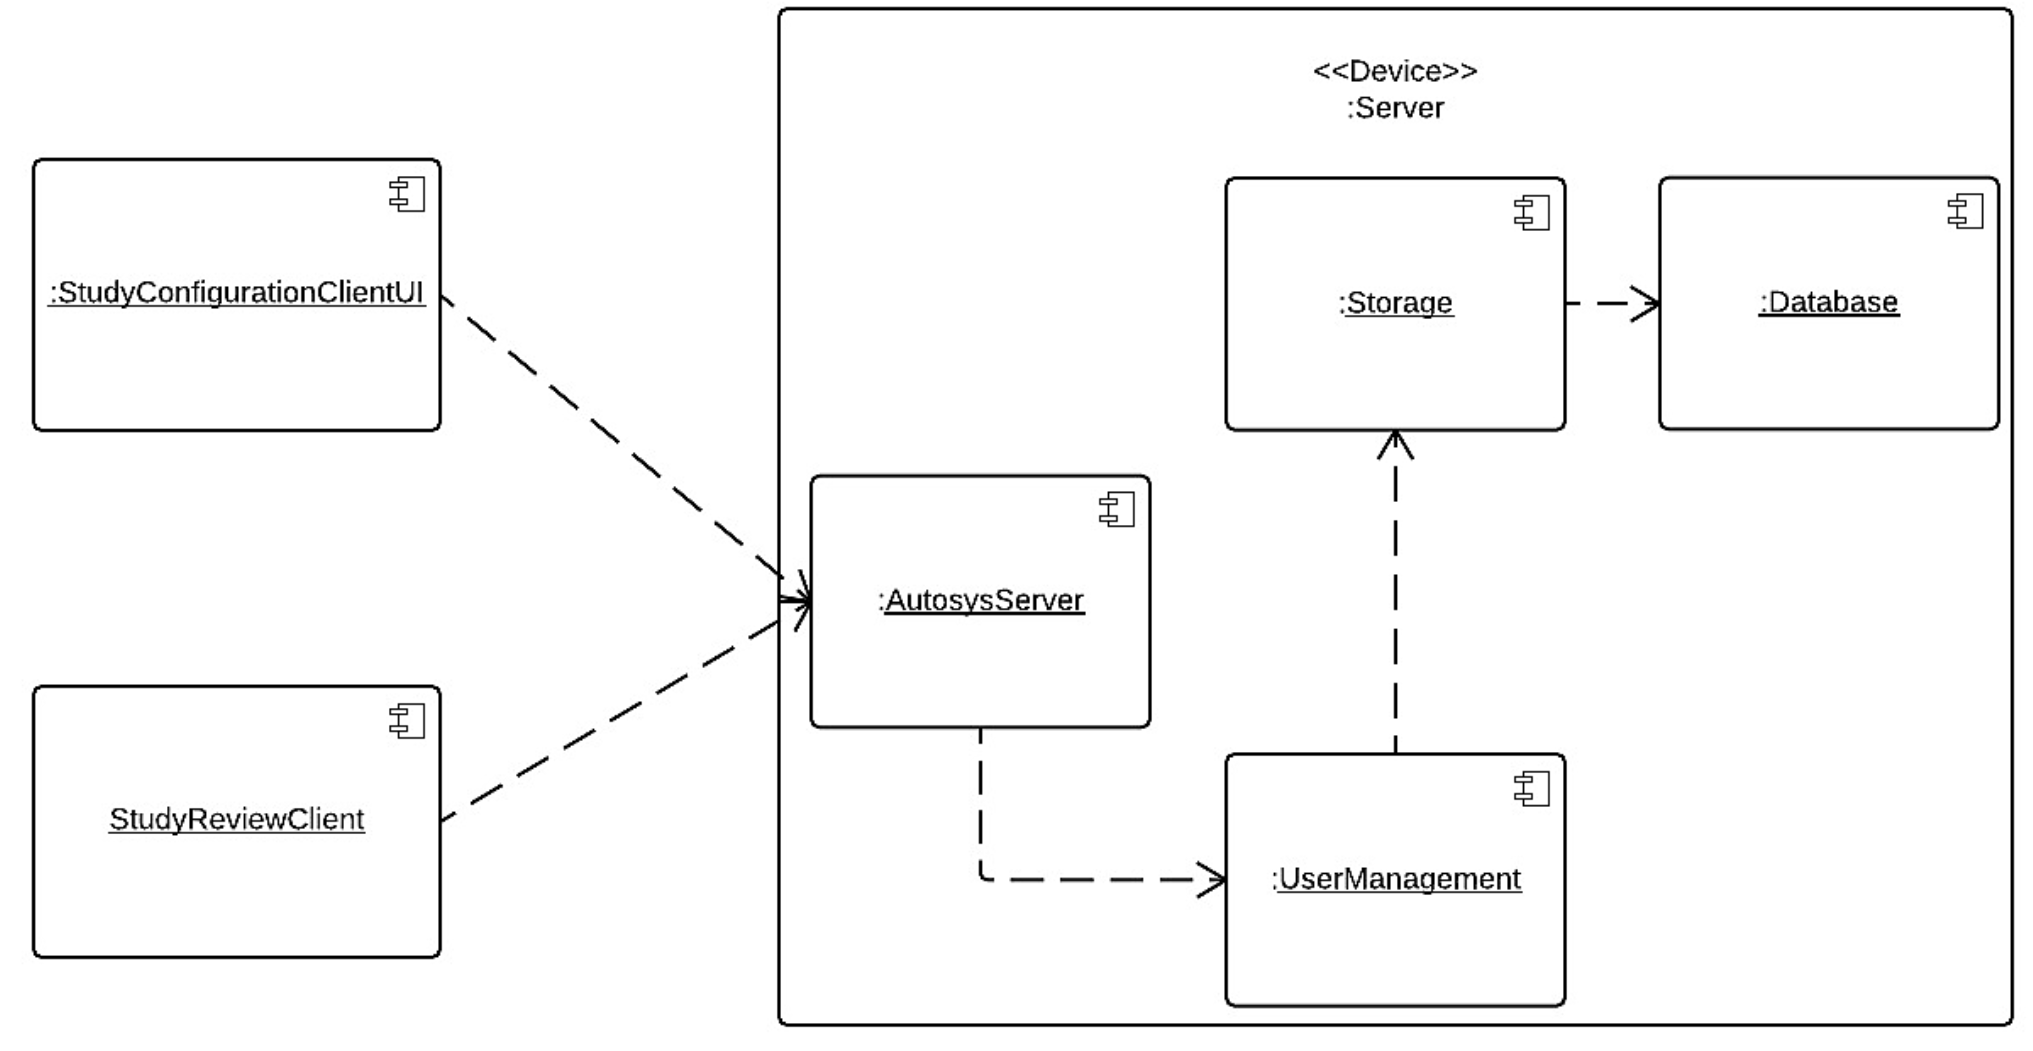
\includegraphics[width=\textwidth]{Images/mappingImage}
\caption{Software mapping of prior subsystem decomposition. Note that the components UserManagement, PaperManagement and StudyManagement has been collapsed into a single unit called UserManagement }
\end{figure}
\paragraph{Program components}\mbox{}\\
The server will be implemented in C Sharp as requested by the the client. By using C Sharp, we can utilise to Microsoft expansive database systems and interfaces especially in regards to the database. Additionally this also make the program easier to maintain, since C Sharp is a well known language and can utilise the .NET framework. As communication between the server and the clients, we plan to communicate with HTTPS  request containing JSON object. This will make it easier to implement future changes and even completely replace the clients user interface with a more modern solution like a web page